\documentclass[border=10pt]{standalone}

\usepackage{tikz}
\usepackage{tikzsymbols}
\usetikzlibrary{calc,patterns,shapes.geometric}

\def\centerarc[#1](#2)(#3:#4:#5){\draw[#1] ($(#2)+({#5*cos(#3)},{#5*sin(#3)})$) arc (#3:#4:#5);}

\begin{document}
	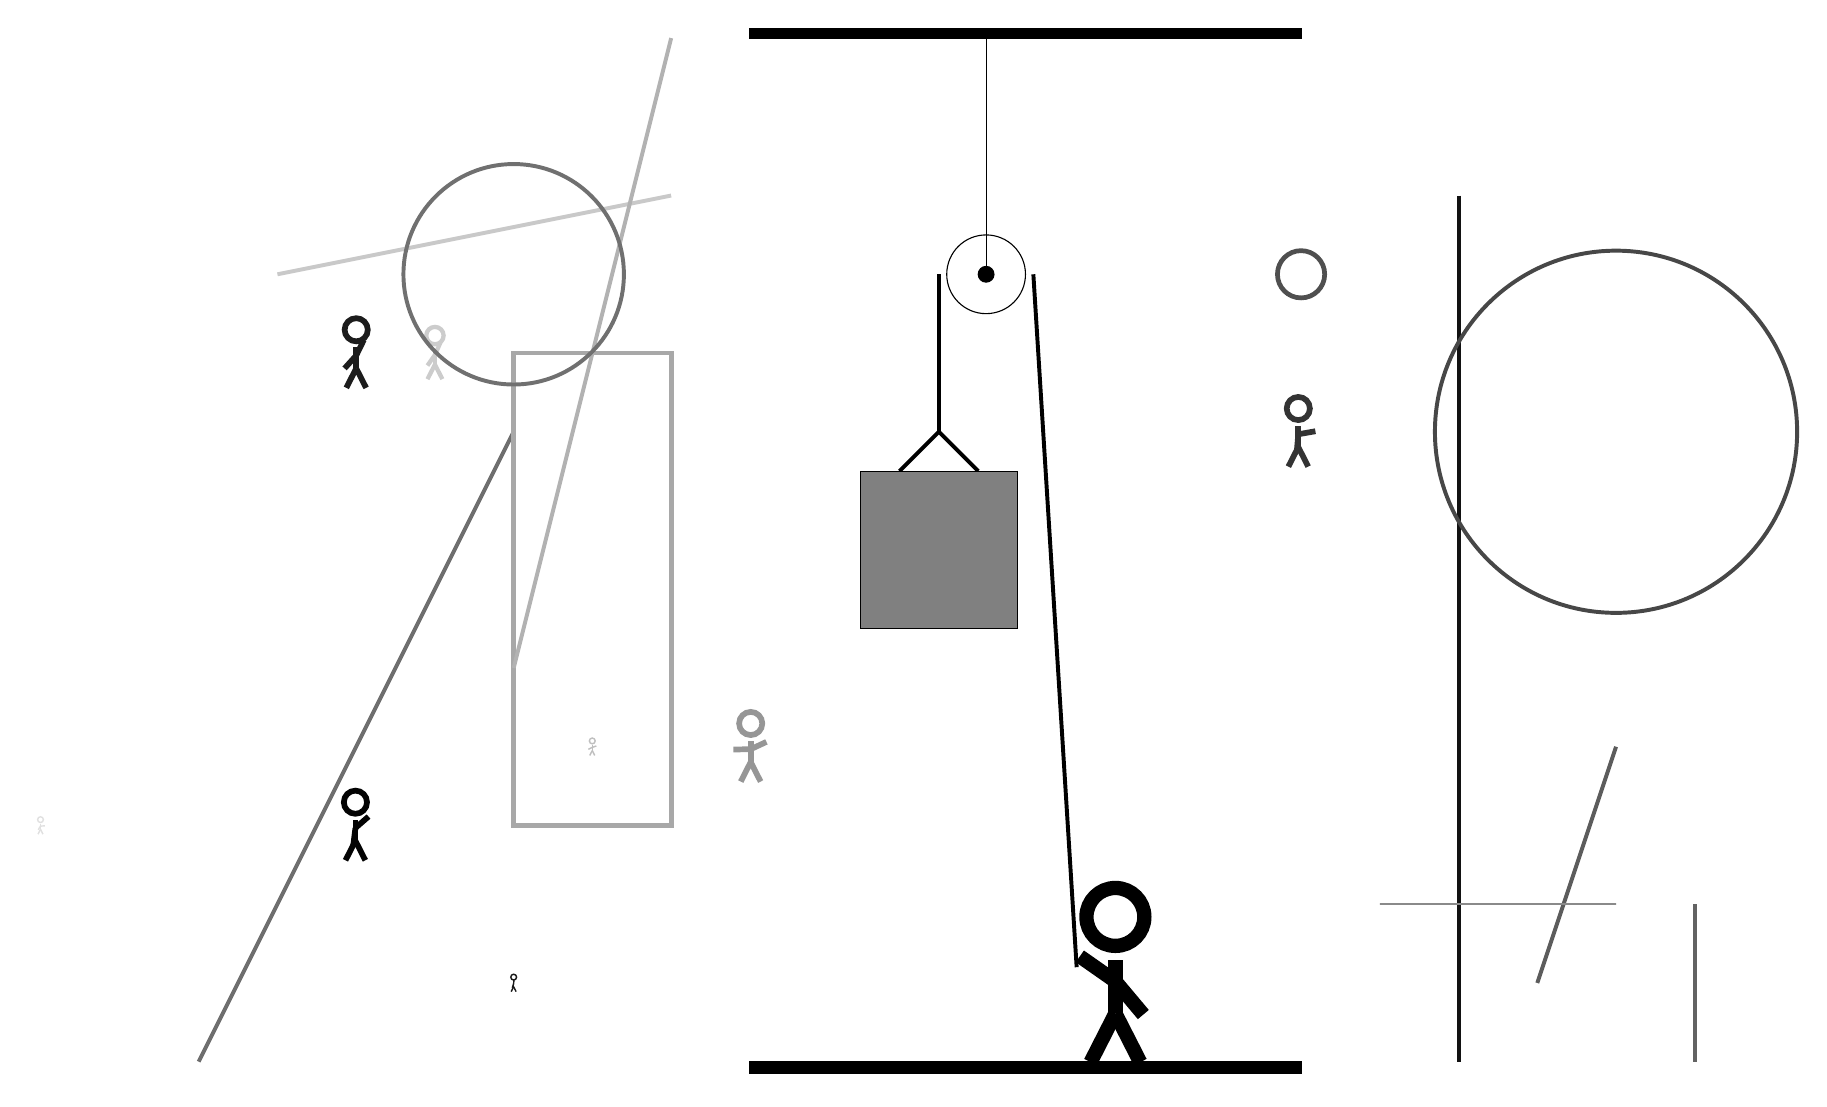
\begin{tikzpicture}
		%%%%% START %%%%%
		
		\draw[fill=black] (-2, 10) rectangle (5, 10.125);
		
		\draw (1, 7) circle (0.5);
		\draw[fill=black] (1, 7) circle (0.1);
		\draw (1, 10) -- (1, 7);
		
		\draw[line width=0.5mm] (-0.1, 4.5) -- (0.4, 5.0) -- (0.9, 4.5);
		\draw[fill=black!50] (-0.6, 4.5) rectangle (1.4, 2.5);
		
		\draw[line width=0.5mm] (0.4, 7) -- (0.4, 5.0);
		\centerarc[line width=0.5mm](1, 7)(0:180:0.6);
		\draw[line width=0.5mm](1.6, 7) -- (2.15, -1.8);
		
		\node at (2.6, -1.9) {\Strichmaxerl[10][-35][-50]};
		
		\node[line width=0.7mm, color=black!25] at (-4, 1) {\Strichmaxerl[1][27][18]};
		
		\node[line width=0.7mm, color=black!80] at (5, 5) {\Strichmaxerl[4][85][10]};
		\node[line width=0.2mm, color=black!20] at (-6, 6) {\Strichmaxerl[3][55][66]};
		\draw[line width=0.5mm, color=black!93](7, 8) -- (7, -3);
		
		\node[line width=0.6mm, color=black!12] at (-11, 0) {\Strichmaxerl[1][58][3]};
		\draw[line width=0.5mm, color=black!21](-3, 8) -- (-8, 7);
		
		\draw[line width=0.5mm, color=black!64](9, 1) -- (8, -2);
		\draw[line width=0.5mm, color=black!57](-5, 5) -- (-9, -3);
		\draw[line width=0.6mm, color=black!34] (-3, 6) rectangle (-5, 0);
		
		\node[line width=0.6mm, color=black!90] at (-5, -2) {\Strichmaxerl[1][72][86]};
		\draw [line width=0.5mm, color=black!72](9, 5) circle (2.3);
		\node[line width=0.3mm, color=black!89] at (-7, 6) {\Strichmaxerl[4][48][64]};
		\draw [line width=0.7mm, color=black!14](-4, -2) circle (0.0);
		
		\draw [line width=0.6mm, color=black!69](5, 7) circle (0.3);
		\draw[line width=0.5mm, color=black!30](-5, 2) -- (-3, 10);
		\node[line width=0.5mm, color=black!41] at (-2, 1) {\Strichmaxerl[4][1][25]};
		
		\node[line width=0.3mm, color=black!99] at (-7, 0) {\Strichmaxerl[4][83][41]};
		\draw [line width=0.5mm, color=black!56](-5, 7) circle (1.4);
		\draw[line width=0.2mm, color=black!46] (6, -1) rectangle (9, -1);
		\draw[line width=0.5mm, color=black!61](10, -3) -- (10, -1);
		
		\draw[fill=black] (-2, -3) rectangle (5, -3.15);
		
		%%%%% END %%%%%
	\end{tikzpicture}
\end{document}